%%%%%%%%%%%%%%%%%%%%%%%%%%%%%%%%%%%%%%%%%%%%%%%%%%%%%%%%%%%%%%%%%%%%%%
%%  dissertation.tex, to be compiled with latex2e.                   %
%%  16 April 2012                                                    %
%%%%%%%%%%%%%%%%%%%%%%%%%%%%%%%%%%%%%%%%%%%%%%%%%%%%%%%%%%%%%%%%%%%%%%
%%                                                                   %
%%  Writing a Doctoral Dissertation with LaTeX at                    %
%%           Georgia State University                                %
%%                                                                   %
%%  (Running this ``template'' will generate the documentation.)     %
%%                                                                   %
%%%%%%%%%%%%%%%%%%%%%%%%%%%%%%%%%%%%%%%%%%%%%%%%%%%%%%%%%%%%%%%%%%%%%%

\documentclass[12pt,gsu,online,openany,hidelinks]{gsudiss}
% Remove the option "online" to produce a print version (page number at the center of the footer)

\usepackage{natbib}
% \usepackage{subfigure}                % To format bibliographies.
\setlength{\bibsep}{0pt}           % Necessary for bib entries to have
                                   % correct line spacing.

\usepackage[hidelinks]{hyperref}
\hypersetup{
    colorlinks=false,
    pdfborder={0 0 0},
}

% Here is how you set the fonts for each section of the TOC
\usepackage{tocloft}
\renewcommand{\cftfigfont}{Figure\ }
\renewcommand{\cfttabfont}{Table\ }
\renewcommand{\cftchapfont}{\bfseries}  % Set the font for the chapters in TOC
\renewcommand{\cftsecfont}{\normalfont} % Set the font for the sections in TOC, e.g., you can change it to \renewcommand{\cftsecfont}{\bfseries}
\renewcommand{\cftsubsecfont}{\normalfont}  % Set the font for the subsections in TOC, e.g., you can change it to \renewcommand{\cftsubsecfont}{\bfseries\itshape}{\bfseries}
\renewcommand{\cftsubsubsecfont}{\itshape}  % Set the font for the subsubsections in TOC
\renewcommand{\cftparafont}{\mdseries}  % Set the font for the paragraphs in TOC

\setcounter{tocdepth}{2}      % The depth of table of contents, the setting of 2 means it only goes to subsections, you can change it (e.g. 3 is to include subsubsections).


\usepackage{lscape}
\usepackage{geometry}
\usepackage{array}
\usepackage{deluxetable}
\usepackage{longtable,ltcaption}
\usepackage{float}
\usepackage[caption = true]{subfig}
% The ltcaption package supports \CaptionLabelFont & \CaptionTextFont
% introduced by the NTG document classes
\renewcommand\CaptionLabelFont{\normalsize}
\renewcommand\CaptionTextFont{\normalsize}

\usepackage{amsmath,amsthm,amsfonts,amsopn,amssymb} % Some nice math packages.
\usepackage{eucal}                 % Euler fonts for equations.
\usepackage{verbatim}              % Allows quoting source with commands.
\usepackage{graphicx}              % For powerful manipulation of figures.
\usepackage{ctable}                % My preference table package.
\usepackage[overlay]{textpos}      % Put stuff anywhere, I mean anywhere ...
\usepackage{pstricks}              % Draw stuff especially on top figures etc...
\usepackage{afterpage}             % Useful for absolute placement of figures and tables.
\usepackage{longtable}             % for 'longtable' environment
\usepackage{pdflscape}             % for 'landscape' environment
\usepackage{fancyvrb}              % for verbatim environments (see usercommands.tex)

\usepackage{float}
\floatstyle{boxed}
\newfloat{code}{h}{ext}
\floatname{code}{Code}

\usepackage{atbeginend}            % Modify space before and after
                                   % equations. These are my preferences.
\AfterBegin{equation}{\addtolength{\abovedisplayskip}{-0.5\baselineskip}}
\BeforeEnd{equation}{\addtolength{\belowdisplayskip}{-0.5\baselineskip}}
\AfterBegin{equation*}{\addtolength{\abovedisplayskip}{-0.5\baselineskip}}
\BeforeEnd{equation*}{\addtolength{\belowdisplayskip}{-0.5\baselineskip}}

\renewcommand{\topfraction}{0.85}        % These modify figure placement on
\renewcommand{\bottomfraction}{0.85}     % the page and various other space
\renewcommand{\textfraction}{0.10}       % requirements for figures.
\renewcommand{\floatpagefraction}{0.80}  % These 5 lines are not
\renewcommand{\arraystretch}{0.5}        % necessary but I think its better
                                         % than latex default.

\setlength{\tabcolsep}{3pt}        % shrink column spacing so your tables 
                                   % can be wider (yay Todd Tables)
%\setlength{\LTcapwidth}{\textwidth}% so your rotated, normal-sized
                                   % longtable titles won't wrap oddly.


\clubpenalty=1000                  % Make Latex try hard to fix
\widowpenalty=1000                 % "stray lines" in paragraphs,
                                   % i.e. paragraph that begin at the
                                   % last line of a page, or end with
                                   % the last line on the following
                                   % page. This looks silly.
\raggedbottom

\settocname{TABLE OF CONTENTS}              % Set the "Table of Contents"
                                   % name. This is the default. You
                                   % can use "Table of Contents" for example.

\setlofname{LIST OF FIGURES}               % Change the name from 'List of
                                   % Figures'. Use whatever you wish.

\setlotname{LIST OF TABLES}                % Change the name from 'List of
                                   % Tables'. Use whatever suit your
                                   % fancy.

\settocbibname{REFERENCES}         % Change the name from
                                   % 'Bibliography'. Change it back if
                                   % you feel like it.

\setloaname{LIST OF ABBREVIATIONS}
                                   % I Changed the name from 'List of
                                   % Abbreviations'. Use any name that
                                   % makes sense here. If you don't
                                   % have an "abbreviations.tex" file,
                                   % this command will do nothing.

\setfigname{Figure\ }               % Set the caption labels for figures.

\settabname{Table\ }                % Set the caption labels for tables.

\setcapfont{pnc}                   % Set the caption font for
                                   % both tables and figures.

\chapternumsize{\normalsize}            % You can use any standard latex sizes here.
\chapterheadsize{\normalsize}           % You can use any standard latex sizes here.
\chaptertitlesize{\normalsize}           % You can use any standard latex sizes here.
                                   % These defaults look good to me.

\beforechapterheadname{CHAPTER}         % Optional text to put in front of
                                   % the chapter number.
\afterchapterheadname{}          % Optional text to put after the
                                   % chapter number. The default
                                   % looks like this: --1--. Of course
                                   % you can change this to any
                                   % format, for e.g. $\sim$

\chapterheadpos{center}            % You can use 'right', 'left',
                                   % 'center'.

\chaptertitlepos{center}           % You can use 'right', 'left',
                                   % 'center'

\chapterheadverticalspace{-1em}     % The space between the Chapter head
                                   % and the top of page. This distance
                                   % is not absolute, but relative to
                                   % the parameters set by the
                                   % geometry package. Play around
                                   % with this number to suit your needs.

\chapterbetweentitlespace{-1.em}   % The space between the chapter head
                                   % and the title head.

\titleheadverticalspace{2em}       % The space between the title head
                                   % and the text.

\sectiontitlesize{\normalsize}          % This is obvious.
\sectiontitlepos{left}             % Obvious.

\sectiontitleverticalspace{1em}    % The space between the section head
                                   % and the text.

\subsectiontitlesize{\normalsize}       % Obvious.
\subsectiontitlepos{left}          % Obvious.

\subsectiontitleverticalspace{0.5em} % You get the idea...

\subsubsectiontitlesize{\normalsize}
\subsubsectiontitlepos{left}

\subsubsectiontitleverticalspace{0.5em}

\sepabbrev{7em}                    % The space between the abbreviation
                                   % lists, that is, if you have
                                   % one. Has to be >= 5em.

\prettify{pnc}

\printdraft{\textcolor{gray}\small DRAFT}    % In order to use this
                                   % command, you have to enable "drafts"
                                   % in the option of the gsudiss
                                   % class, otherwise it does
                                   % nothing. This prints the word
                                   % "DRAFT" in gray color in the header of your
                                   % dissertation. You can go wild
                                   % here if you want. Just make sure
                                   % you disable the draft option
                                   % before final printing.

\author(FirstName LastName)              % Name required.

\title(Manuscript Title)    % Title of dissertation Required.

\titlesize(12)(12)                               % This is for changing
                                             % the default font size
                                             % for your title. The
                                             % first argument is the
                                             % font size, the second
                                             % is the line spacing for
                                             % long tiles that wrap to
                                             % more than one line.
                                             % Default is equivalent
                                             % to the \LARGE command,
                                             % which is roughly (22)(22).


%%%%%%%%%%%%%%%%%%%%%%%%%%%%%%%%%%%%%%%%%%%%%%%%%%%%%%%%%%%%%%%%
% \committee: The first parenthesis must contain your supervisor name.
%         You can have two supervisors, in which case, the
%         second supervisor goes into the square brackets, next to the
%         first. If you have one like me, then leave the second entry blank, like below. The
%         rest of the parentheses contains the rest of your committee members. You
%         can have up to six entries, NOT including your supervisor(s). My
%         school requires five or four. I have five (5) members
%         below. Note that there is no need to put the "Dr." title in front of any of the names.
% Adjust margins to 1.0in on all sides

\committee(FirstName LastName)[] % Committee CHAIR's First Name Last Name.Only the first and last name of your committee chair should be listed here. Please do not include their titles. In other words, do not list “Dr.” or “Ph.D.” here.
          (FirstName LastName) % Committee MEMBER's First Name Last Name. Only the first and last name of your committee members should be listed here. Please do not include their titles. In other words, do not list “Dr.” or “Ph.D.” here
          (FirstName LastName)
          (FirstName LastName)
          (FirstName LastName)%

\graduationyear(Year)

\graduationmonth(Month) % The Month and Year here must be the month and year of your graduation—not the month and year of your submission or upload.


%%%%%%%%%%%%%%%%%%%%%%%%%%%%%%%%%%%%%%%%%%%%%%%%%%%%%%%%%%%%%%%%%%%%%%
%               The dissertation starts here.                        %
%%%%%%%%%%%%%%%%%%%%%%%%%%%%%%%%%%%%%%%%%%%%%%%%%%%%%%%%%%%%%%%%%%%%%%

\newcommand\arcdeg{\mbox{\ensuremath{^\circ}}}%
\newcommand\arcmin{\mbox{\ensuremath{^\prime}}}%
\newcommand\arcsec{\mbox{\ensuremath{^{\prime\prime}}}}%
\newcommand{\point}{\mbox{\ensuremath{\!\!.}\thinspace}}
\newcommand{\minusone}{\ensuremath{^{-1}}}
\newcommand{\minustwo}{\ensuremath{^{-2}}}
\newcommand{\minusthree}{\ensuremath{^{-3}}}
\newcommand{\minusfive}{\ensuremath{^{-5}}}
\newcommand{\plusthree}{\ensuremath{^{3}}}
\newcommand{\plusfive}{\ensuremath{^{5}}}
\newcommand{\kms}{\mbox{\ km\,s\ensuremath{^{-1}}}}
\newcommand{\fig}{Figure~}
\newcommand{\figs}{Figures~}
\newcommand{\tab}{Table~}
\newcommand{\tabs}{Tables~}
\newcommand{\eqn}{Equation~}
\newcommand{\eqns}{Equations~}
\newcommand{\vracc}{\mbox{$\mathrm{v=kr}$}\xspace}
\newcommand{\vrdec}{\mbox{$\mathrm{v=v_{max}-k^{'}(r-r_t)}$}\xspace}
\newcommand{\vrootracc}{\mbox{$\mathrm{v=k_{1}\sqrt r}$}\xspace}
\newcommand{\vrootrdec}{\mbox{$\mathrm{v=v_{max}-k_{2}\sqrt{r-r_t}}$}\xspace}
\newcommand{\rlaw}{\mbox{$r\ $law}\xspace}
\newcommand{\rootrlaw}{\mbox{$\sqrt r\ $law}\xspace}
\newcommand{\resolvingpower}{\mbox{$\lambda/\Delta\lambda$}\xspace}
\newcommand{\OIII}{\mbox{[\acs{O3}]}\xspace}
\newcommand{\solarmass}{\mbox{\ M\ensuremath{_{\odot}}}}
\newcommand{\arcpt}{${{\lower3pt\hbox{$^{\prime\prime}$}}\atop{\raise4pt\hbox{.}}}$}
\newcommand{\msun}{$M_\odot$}               % You can put some self-defined
                                   % commands in this file like
                                   % math abbreviations, etc.

\begin{document}

%%%%%%%%%%%%%% The title, abstract and front matters %%%%%%%%%%%%%%%

\pagestyle{empty}
\begin{center}
Manuscript Title % Your title should be in title caps.

%%%%%%%%%%%%%%%%
% If it takes more than two lines, it must be double-spaced, for example,

% Manuscript Title line 1
% \vspace*{.1in}
% Manuscript Title line 2
%%%%%%%%%%%%%%%%

\vspace{1.4in}
by\\
\vspace{1.4in}
First and Last Name\\ %Your name should be in title caps.
\vspace{1.4in}
Under the Direction of Committee Chair's Name, MA/Ph.D. \\ %List your supervisor's first and last name followed by their letter credentials. Do not put their title before their name.
\vspace{1.4in}
A Thesis/Dissertation Submitted in Partial Fulfillment of the Requirements for the Degree of\\  % Choose either thesis or dissertation and delete the other.
\vspace{.2in}
Level and Degree Title \\ % Your degree does not include your specialization. The following are your options: Master of Arts, Master of Science, or Doctor of Philosophy. Do NOT list your department/field here.
\vspace{.2in}
in the College of Arts and Sciences \\
\vspace{.2in}
Georgia State University \\
\vspace{.2in}
Year

\end{center}

\pagebreak 


\begin{center}
    ABSTRACT\\ 
\end{center}

\doublespacing
The abstract paragraph is mandatory. Start the abstract paragraph here. Double-space this paragraph. Limit the abstract of a thesis to 150 words. Limit the abstract of a dissertation to 350 words. ``Your abstract will not be accepted if it exceeds the limit by even one word.''

\begin{singlespace}
\vfill   
\vspace{0.5in}
\noindent INDEX WORDS:
\hspace{0in}
\parbox[t]{4.5in}{
Sample keyword, Sample keyword, Sample keyword}  %It is recommended that you list six keywords. Please use my capitalization here as an example. Should be single-spaced.
\end{singlespace}             % See the TitleAbstract.tex file
%%%%%%%%%%%%%%%%%%%% The front matter of your document %%%%%%%%%%%%%%%%%%%%

\frontmatter
% Copyright page (required), approval page (required), dedication (optional), acknowledgments (optional), table of contents (required), list of tables(required and generated automatically if tables used), list of figures (required and generated automatically if figures used), list of abbreviations (optional), Preface (optional) 

% The title page is required. But you don't need to change anything here. To edit your name and year, please go to file `main.tex'
\copyrightpage

% The approval page is required. But you don't need to change anything here. To edit the committee and other information, please go to file `main.tex'
\approvalpage

% The dedication page is optional. You can write your dedication in `./FrontMatters/dedication.tex' file. Delete that file if you don't want to include it.
\dedicationpage              % This command does nothing if you don't
                             % have a `dedication.tex' file, otherwise
                             % the file is included in the frontmatter.


% The acknowledgment page is optional. You can write your acknowledgment in `./FrontMatters/acknowledgment.tex' file. Delete that file if you don't want to include it.
\acknowledgmentpage          % This command does nothing if you don't
                             % have an `acknowledgment.tex' file, otherwise
                             % the file is included in the frontmatter.

\tableofcontents             % Table of Contents will be automatically
\clearpage                   % generated and placed here.

\listoftables                % List of Tables will be automatically
\clearpage                   % generated if you had made proper table captions.

\listoffigures               % List of Figures will be automatically
\clearpage                   % generated if you had made proper figure captions.

% The list of abbreviations is optional. You can write your list of abbreviations in `./FrontMatters/abbreviations.tex' file. Delete that file if you don't want to include it.
\listofabbreviations         % List of Abbreviations will be
\clearpage                   % automatically generated if you had made any,
                             % following the style of the "Acronym"
                             % package. See my "abbreviation.tex" file
                             % for example usage. If you don't have
                             % this file, the command does nothing.
              % See the frontmatter.tex file

%%%%%%%%%%%%%%%%%%%% The main chapters %%%%%%%%%%%%%%%%%%%%%

\pagestyle{plain}
\mainmatter                        % Main chapters starts here

\chapter{CHAPTER 1 TITLE}

\section{The First Section of the First Chapter}
	You should probably introduce some stuff here
    
    You should look at the gsudiss.cls file first when you want to change things in how the document is laid out (also, the `Copyright by Your Name' bit is hard-coded there, so you'll have to change that).

\subsection{Your Subsection Title Here}
You should probably introduce some stuff here.

You should look at the gsudiss.cls file first when you want to change things in how the document is laid out (also, the `Copyright by Your Name' bit is hard-coded there, so you'll have to change that).

\subsubsection{Your Subsubsection Title Here}
This is the content for the subsubsection.

\chapter{CHAPTER 2 TITLE}

Hooray for Chapter 2!!!

Sample Figures and Tables below.

And as an example of citing things, I'm going to cite one of our paper~\cite{LAC_first}. 

See \verb|bibliography.bib| for doing references.

\begin{figure*}
	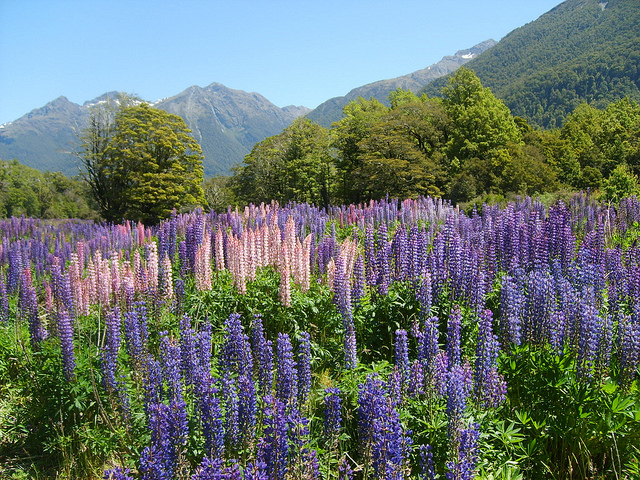
\includegraphics[height =5in]{./Plots/nature.jpg}
	\caption{An individual figure!}
\end{figure*}
        
\begin{figure*}[h]
	\subfloat[\label{fig:HD8538_ellplot}]{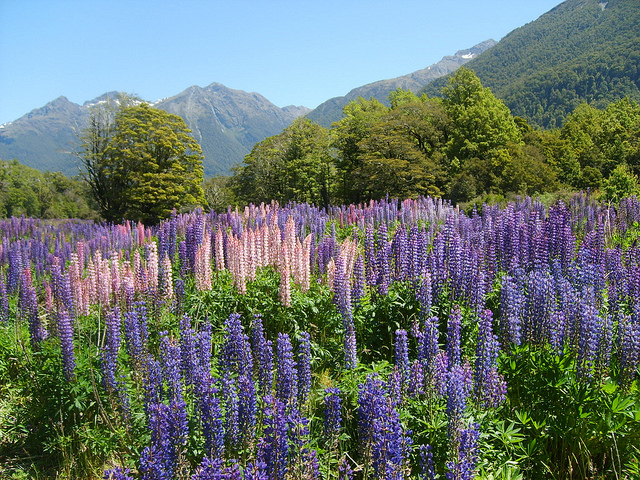
\includegraphics[height =2.5in]{./Plots/nature.jpg}} 
	\subfloat[\label{fig:HD8538_phot}]{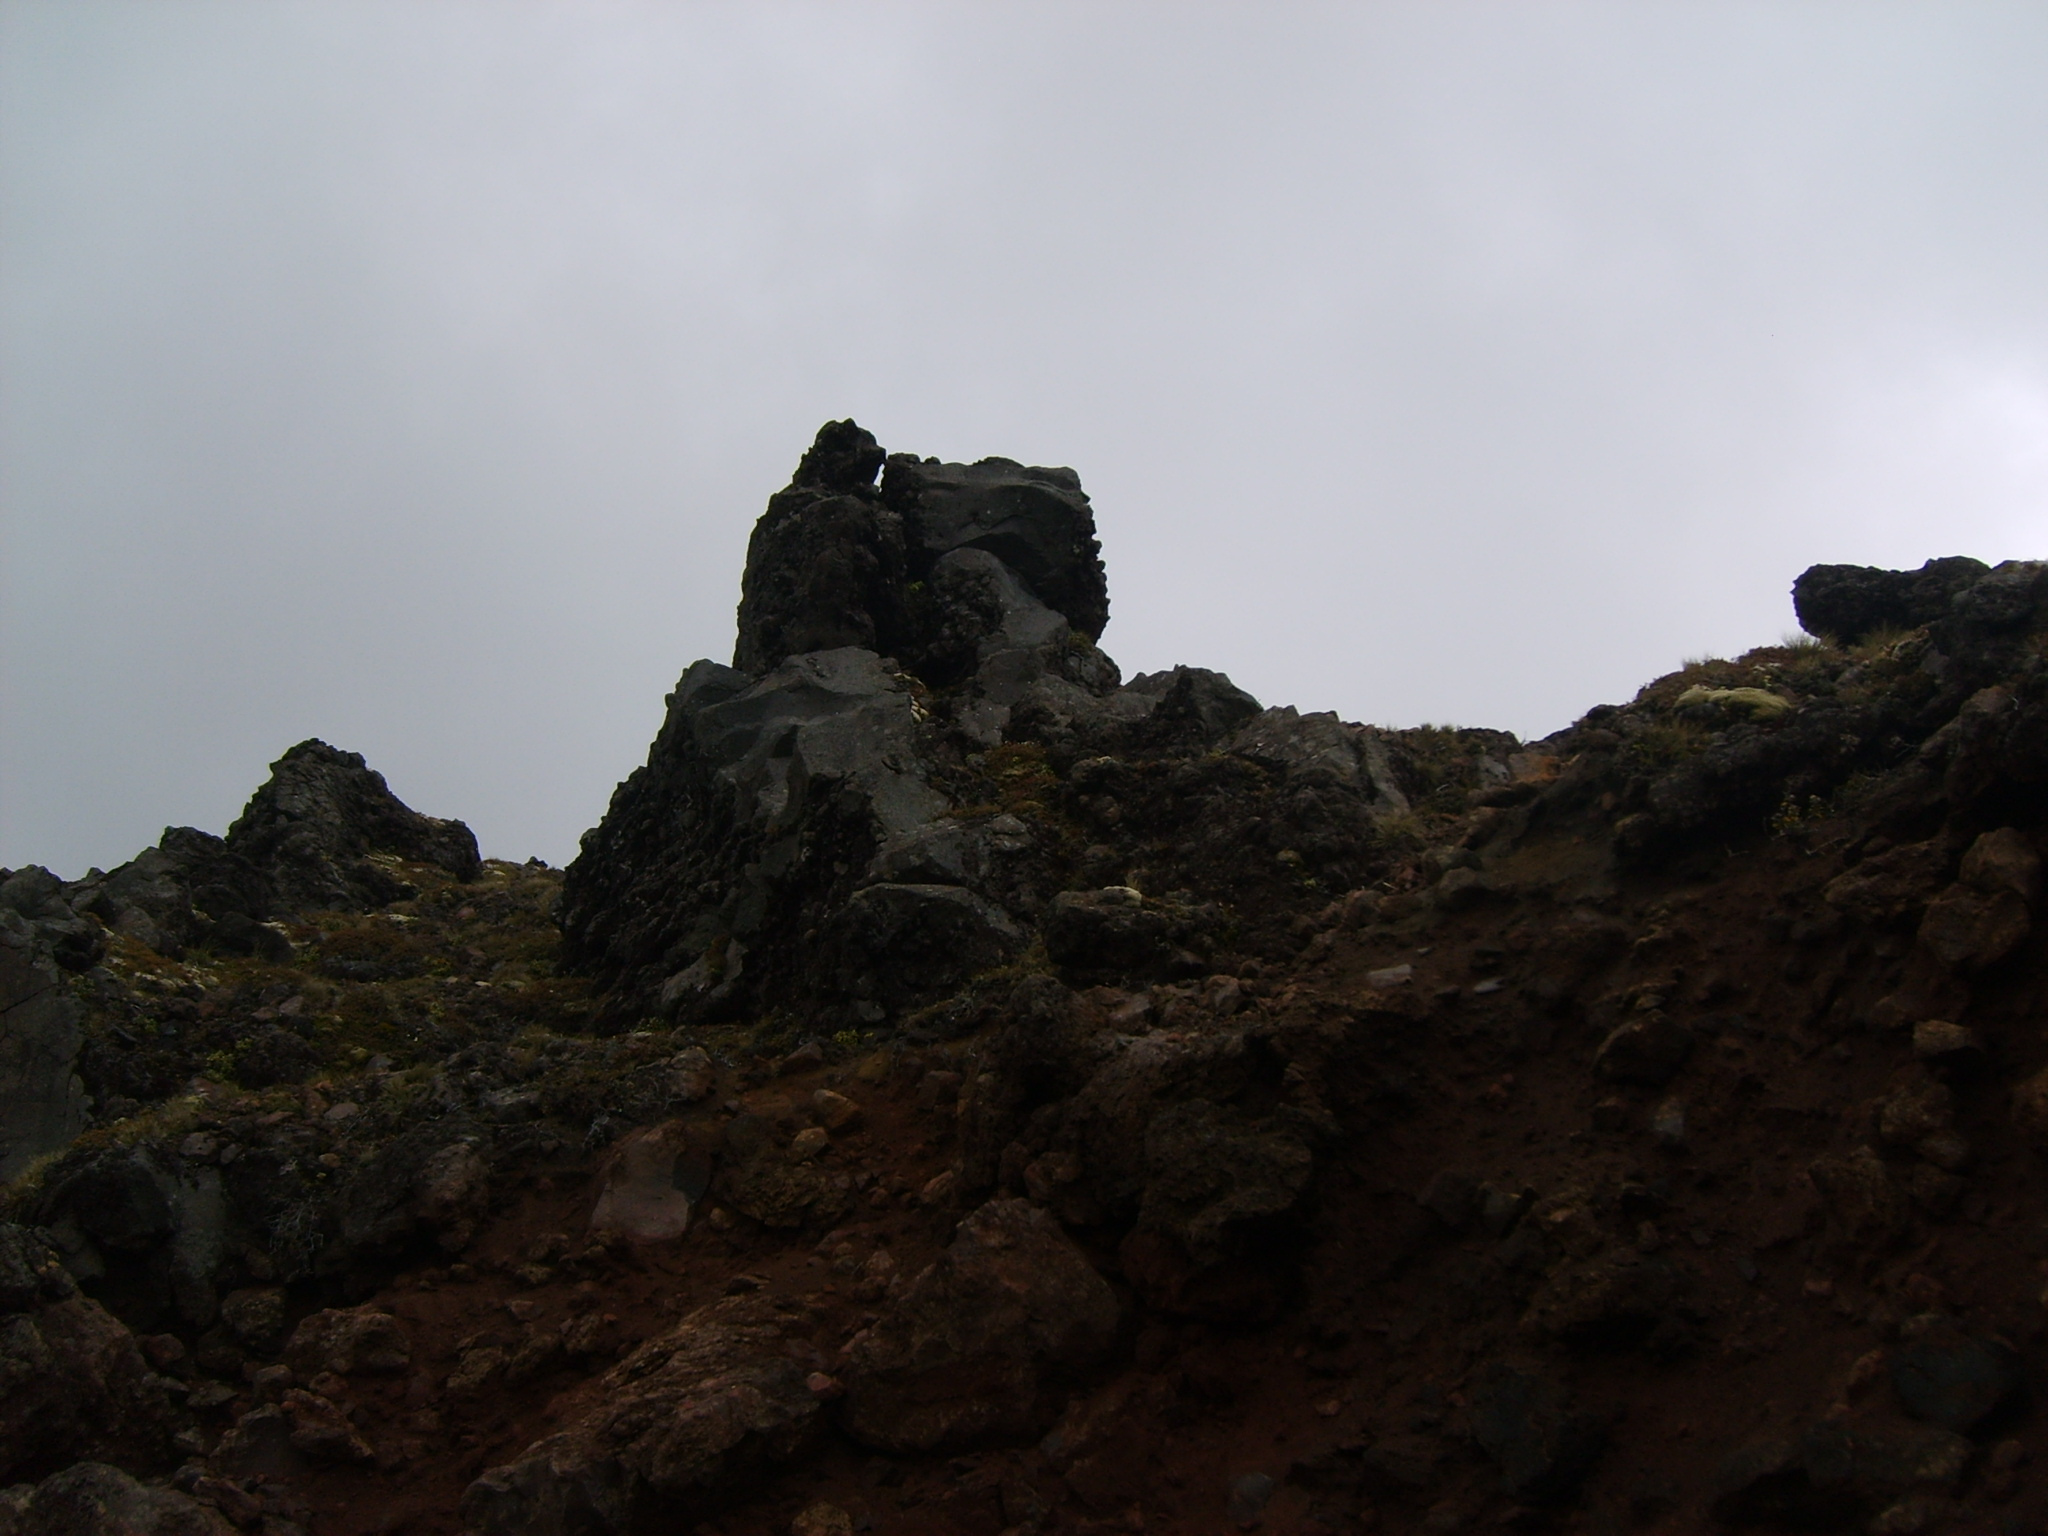
\includegraphics[height =2.5in]{./Plots/rocks.jpg}} \\
	\subfloat[\label{fig:HD8538_vis}]{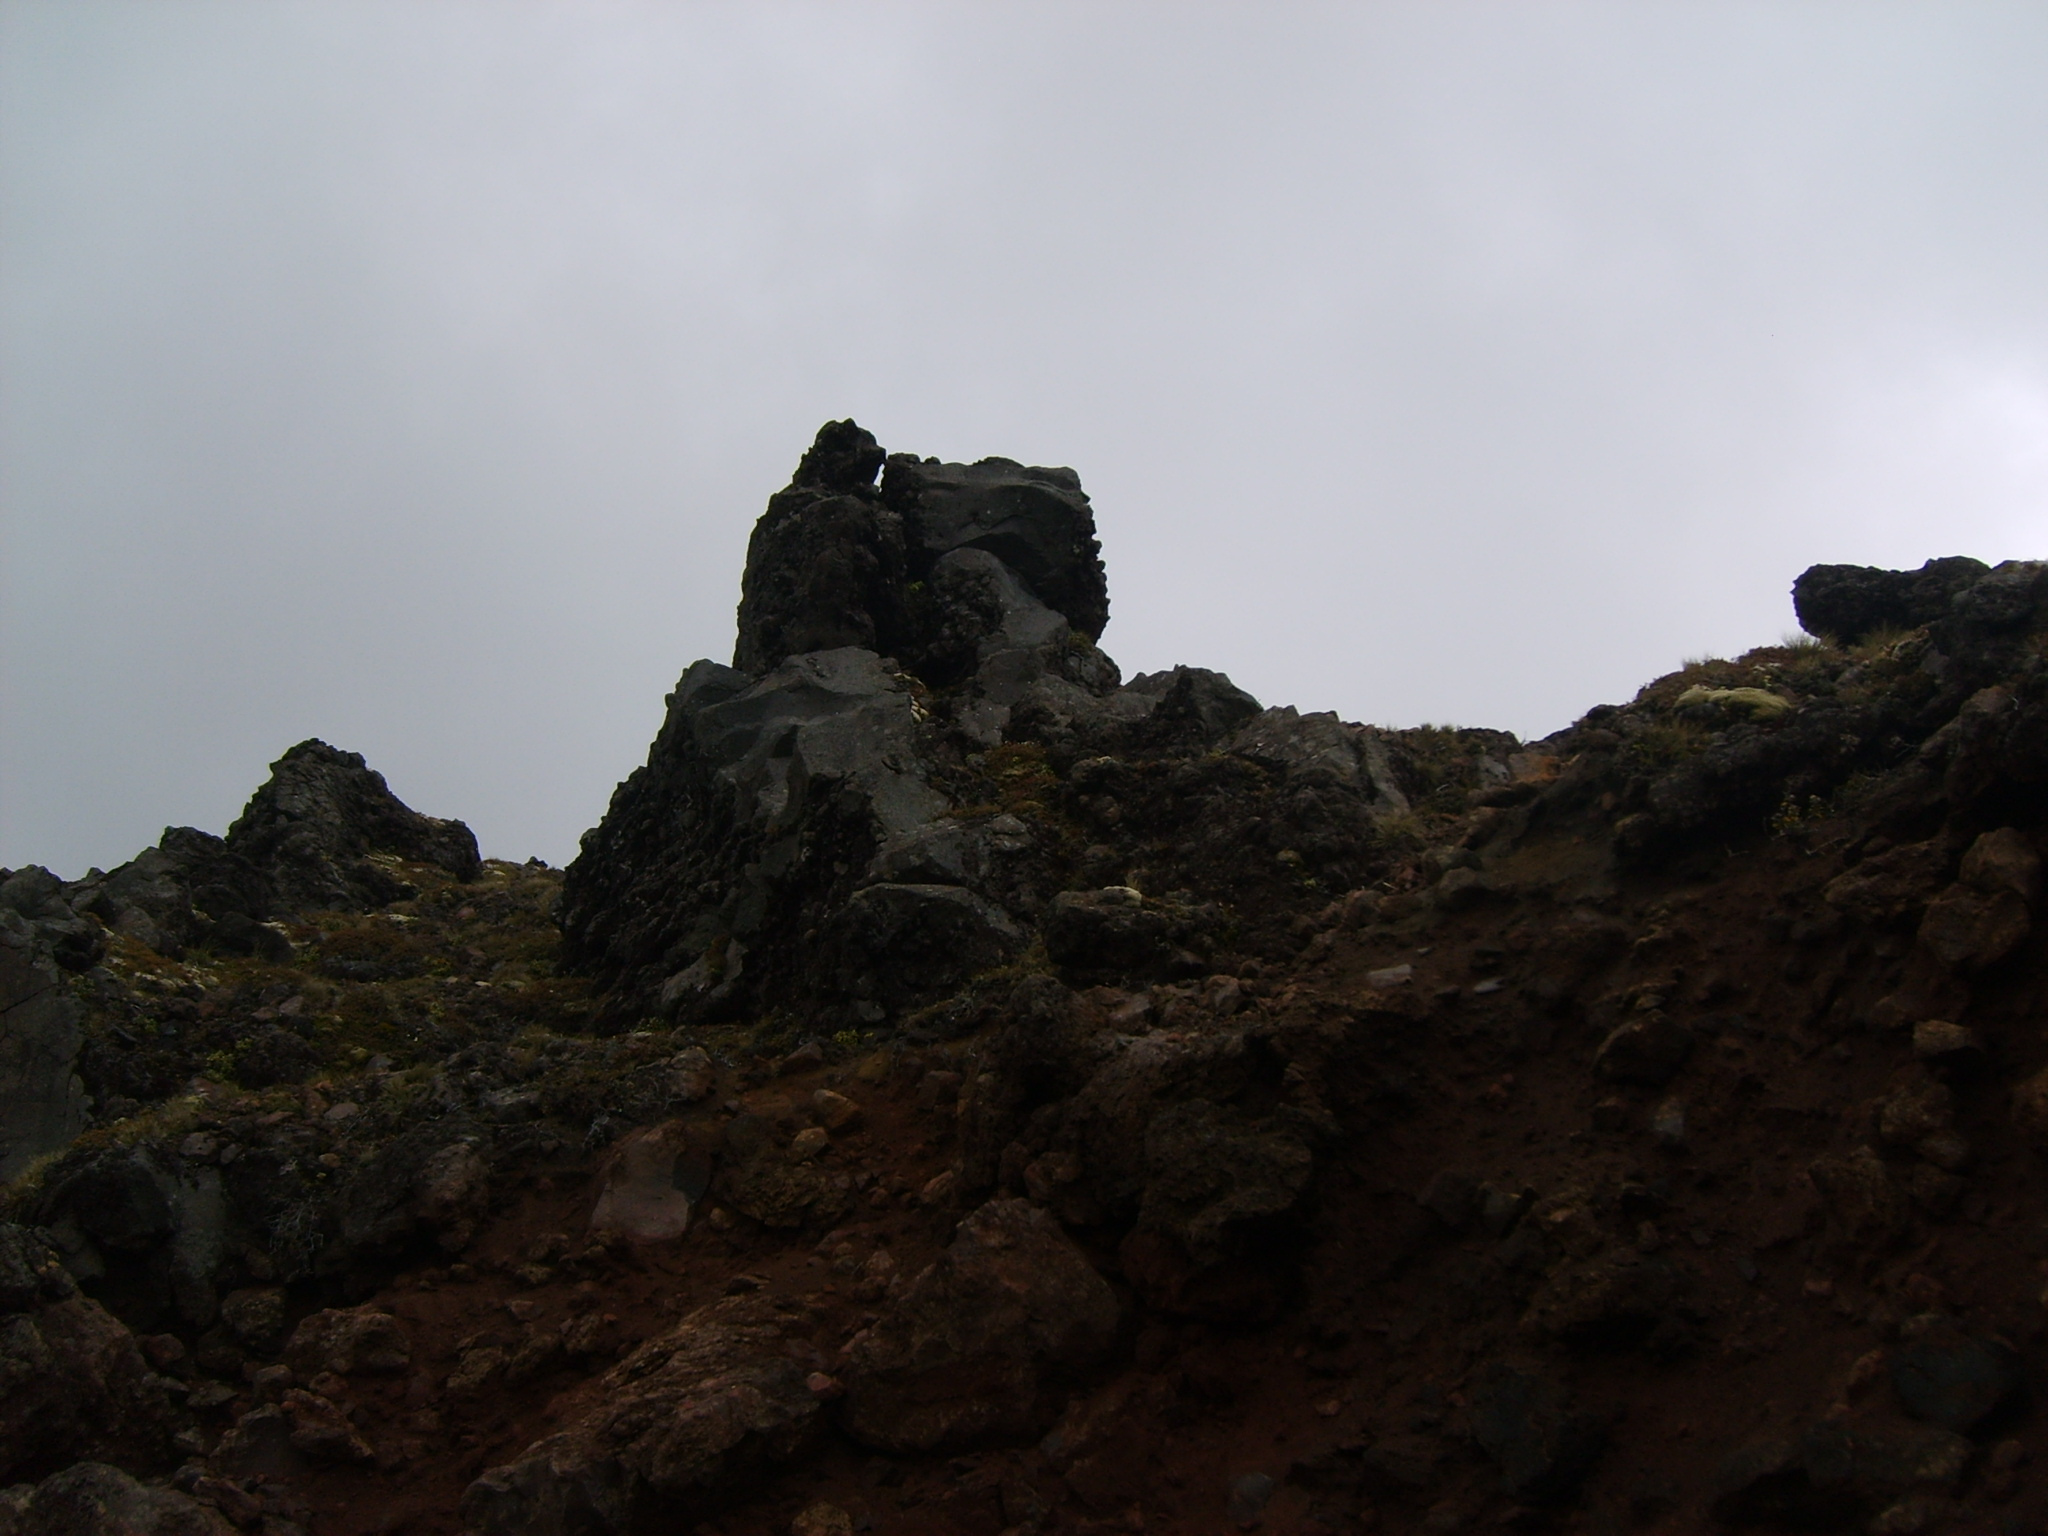
\includegraphics[height =2.5in]{./Plots/rocks.jpg}}
	\subfloat[\label{fig:HD8538_HRD}]{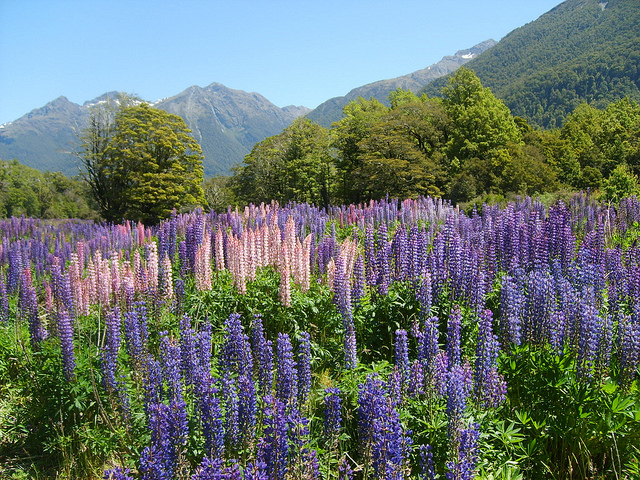
\includegraphics[height =2.5in]{./Plots/nature.jpg}}
	\caption{Multiple figures!}
\end{figure*}



\begin{landscape}
\begin{longtable}{cccccccccccccc}
\label{tab:disk}\\
\caption{Insert Table Caption here}\\
\hline\endhead  % header material
\hline\endfoot  % footer material
\hline
Blah & Blah & Blah \\
\hline
Stuff & Things & etc. \\
\nodata & \nodata & \nodata \\
\end{longtable}
\end{landscape}

\chapter{CHAPTER 3 TITLE}


%%%%%%%%%%%%%%%%%%%% The back matters %%%%%%%%%%%%%%%%%%%%%

\appendix

% Use this file if you have only one appendices. If you have more than one appendix, use Appendices.tex instead
% If you want to write multiple sections in the appendix, it's better also use Appendices.tex 

\chapter*{APPENDIX}
\label{chap:appendix}
\addcontentsline{toc}{chapter}{APPENDIX}

This is the appendix! You can actually have a phantom section in the appendix like the following and refer to it in your text like this: \hyperref[sec:appendix_phantom_section]{Appendix}.

\phantomsection
\section*{A phantom section title in the appendix}
\label{sec:appendix_phantom_section}

However, you probably want to use \verb|Appendices.tex| instead of this file if you really have multiple appendices instead of separating phantom sections.
 % Use this file if you have only one appendix.
% % Use this file if you have more than one appendices. If you have only one appendix, use Appendix.tex instead.

\chapter*{APPENDICES}
\addcontentsline{toc}{chapter}{APPENDICES}

\section{Something}
This is the appendix!

\subsection{First subsection}
Explain some more details here.


\section{Something Else}
Another appendix! % Use this file if you have more than one appendices.


% The bibliography starts here.
% Format the entries according to your department or discipline’s choice of style manual.

\bibliographystyle{plain}           % Please learn to use the
                                    % formatting of Latex's Bibtex. It
                                    % will make your life easier.
\bibliography{mybibliography.bib}   % "mybibliography.bib" contains some
                                    % reference examples.

%%%%%%%%%%%%%%%%%%%%%%%%%%%%%%%%%%%%%%%%%%%%%%%%%%%%%%%%%%%%%%%%%%%%%%
%               The dissertation ends here.                          %
%%%%%%%%%%%%%%%%%%%%%%%%%%%%%%%%%%%%%%%%%%%%%%%%%%%%%%%%%%%%%%%%%%%%%%

\end{document}